\begin{frame}{Nitrogen Vacancy Center (Dangling bonds)} %{{{1
  \begin{columns}
    \begin{column}{0.5\textwidth}
      \begin{tikzpicture}
        \node at (0,0) {%
            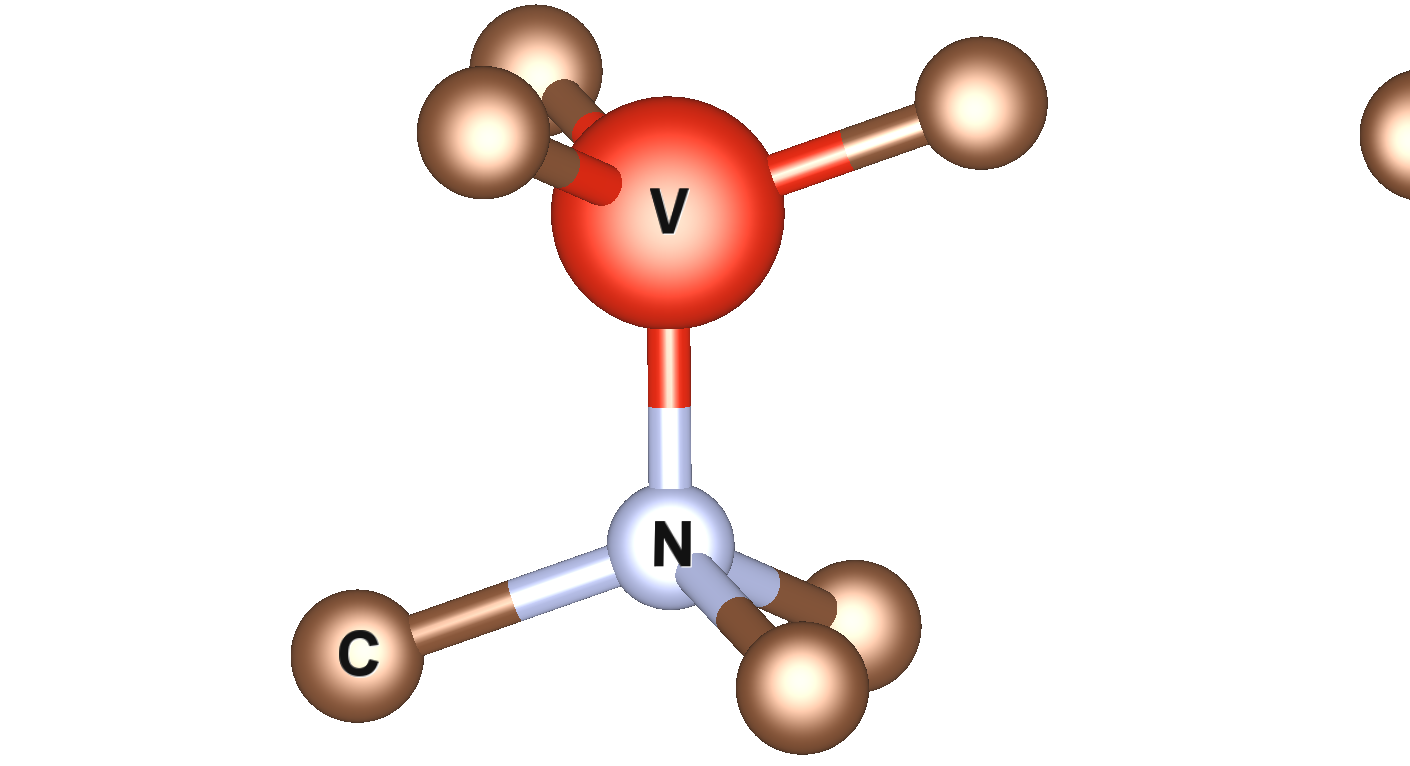
\includegraphics[clip, trim=9cm 0 12cm 0,width=1\textwidth]{images/POSCAR_16_view_defect.png}
          };

        \node at (-0.3,-0.3){%
            $ \sigma _{1} $ 
          };

        \node at (-0.4,1.3){%
            $ \sigma _{2} $ 
          };


        \node at (0.0,2.2){%
            $ \sigma _{3} $ 
          };

        \node at (1.3,2.0){%
            $ \color{black}\sigma _{4} $ 
          };

      \end{tikzpicture}
    \end{column}
    \begin{column}{0.5\textwidth}
      \begin{itemize}
        \item
          Model for the defect 4 $ sp^{3} $ dangling bonds
          $ \left \{ \sigma_{1}, \ldots, \sigma _{4} \right \} $
        \item
          Linear Combination of Atomic Orbitals (LCAO) to
          account for $ C_{3v} $ symmetry.
        \item
          6  electrons for $ \mathsf{NV}^{-} $.
        \item
          From $ \sigma _{i} $ we obtain 4 levels $ a_1(1), a_1(2), e(1), e(2) $
          classified according to their symmetry.

      \end{itemize}
    \end{column}
  \end{columns}

\end{frame}

